% Original finite-coordinate teaching diagram, not a geometric model of C^d.
\documentclass[tikz,border=4mm]{standalone}
\begin{document}
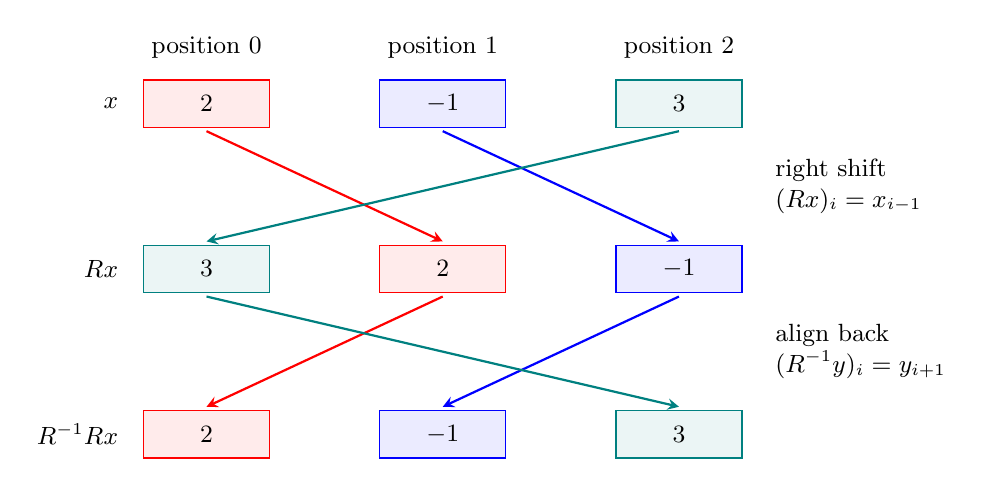
\begin{tikzpicture}[>=stealth,font=\small]
\foreach \x/\value/\color in {0/2/red,3/-1/blue,6/3/teal} {
  \node[draw=\color,fill=\color!8,minimum width=1.6cm,minimum height=.6cm] at (\x,0) {$\value$};
}
\foreach \x/\value/\color in {0/3/teal,3/2/red,6/-1/blue} {
  \node[draw=\color,fill=\color!8,minimum width=1.6cm,minimum height=.6cm] at (\x,-2.1) {$\value$};
}
\foreach \x/\value/\color in {0/2/red,3/-1/blue,6/3/teal} {
  \node[draw=\color,fill=\color!8,minimum width=1.6cm,minimum height=.6cm] at (\x,-4.2) {$\value$};
}
\node[left] at (-1,0) {$x$};
\node[left] at (-1,-2.1) {$Rx$};
\node[left] at (-1,-4.2) {$R^{-1}Rx$};
\foreach \x/\i in {0/0,3/1,6/2} \node[above] at (\x,.45) {position $\i$};
\draw[->,thick,red] (0,-.35)--(3,-1.75);
\draw[->,thick,blue] (3,-.35)--(6,-1.75);
\draw[->,thick,teal] (6,-.35)--(0,-1.75);
\draw[->,thick,red] (3,-2.45)--(0,-3.85);
\draw[->,thick,blue] (6,-2.45)--(3,-3.85);
\draw[->,thick,teal] (0,-2.45)--(6,-3.85);
\node[right,align=left] at (7.1,-1.05) {right shift\\$(Rx)_i=x_{i-1}$};
\node[right,align=left] at (7.1,-3.15) {align back\\$(R^{-1}y)_i=y_{i+1}$};
\end{tikzpicture}
\end{document}
